\documentclass[11pt,a4paper,titlepage]{report}
\usepackage[latin1]{inputenc}
\usepackage{amsmath}
\usepackage{amsfonts}
\usepackage{amssymb}
\usepackage{graphicx}
\usepackage[section]{placeins}
\usepackage{float}
\usepackage{url}
\author{MERMET Alexis}
\title{Bachelor Project: Augmenting Pyrooacooustics with machine learning utilities}
\date{June 8, 2018}

\begin{document}
\maketitle
\tableofcontents
\newpage
%...
\chapter{Introduction}
\section{Objectives of the project}
\hspace*{0.6cm}

During this project, we want to implement new functionalities to the already existing python library, Pyroomacoustics. These functionalities involve machine learning. To this we also have to create wrappers to popular speech datasets as the GoogleSpeechCommand dataset that we will see later. Finally we want to test some signal processing algorithms with a trained neural network.
\section{What is Pyroomacousticsc?}

\hspace*{0.6cm}
First of all Pyroomacoustics is a library allowing us to make audio room simulation  and also apply array processing algorithm in Python. Created at the EPFL by Robin Scheibler, Eric Bezzam and Ivan Dokmanic, this library wants to be an "intuitive python oriented interface to quickly construct different simulation scenarios involving multiple sound sources and microphones in 2D or 3D rooms".\\
\\
\hspace*{0.6cm} 
Before the start of this project, we could find three main classes in Pyroomacoustic: The Room class, the SoundSource class and the MicrophoneArray class. Quickly after I began working, Robin Schleiber also added a Dataset class that helped me to start creating a wrapper.\\
\\
\hspace{0.6cm}
In the Room class you create an object that is a collection of Wall objects, a MicrophoneArray and a list of SoundSource(s). It can be either 2D or 3D.
A SoundSource object has as attributes the location of the source itself and also all of its images sources. In general we create this list directly in the Room object that contains the source.
Finally the MicrophoneArray class consist of an array of microphone locations together with a sampling frequency.
\begin{figure}
	\centering
	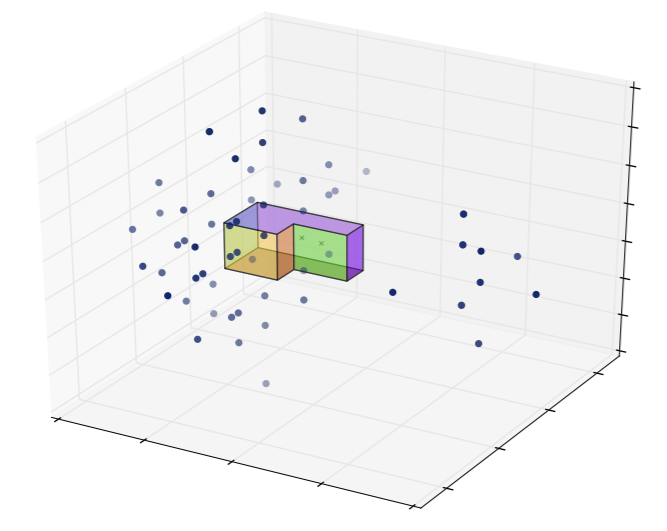
\includegraphics[width=0.7\linewidth]{rapport1}
	\caption[Example of a room in Pyroomacoustic]{Example of a room in Pyroomacoustic}
\end{figure}

\section{What is Tensorflow?}
\hspace*{0.6cm}
As they say on their website, Tensorflow is an "open source software library for high performance numerical computation". We followed a Tensorflow tutorial called "Simple Audio Recognition" to create the neural networks we used during the all project (we are going to explain how it was created in 2.1). We also have reimplement some of their functions to be able to label our sound in the way we want (see 3.2).
\chapter{Theoretical knowledge}
\section{Training the Neural Network}
\hspace*{0.6cm}
In this section we're going to talk about how the neural network was trained. First off all, we download the GoogleSpeechCommand dataset since we use it: to train our network but also afterwards to test the efficiency of our algorithms. This model is considered really simple but is also "quick to train and easy to understand".\\
\hspace*{0.6cm}
This model works as a convolutional network (in fact this model is similar to the one you can use to do some image recognition). First of all a window of time is defined and the audio signal is converted to an image into that window. This is done by "grouping the incoming audio samples into short segments and calculating the strength of the frequencies across a set of bands". All the frequency strengths of a given segment will then be treated as a vector of values. These vectors are then ordered according to the time, forming a two-dimensional array that we will treat as as \underline{spectrogram}\\
\begin{figure}[h]
	\centering
	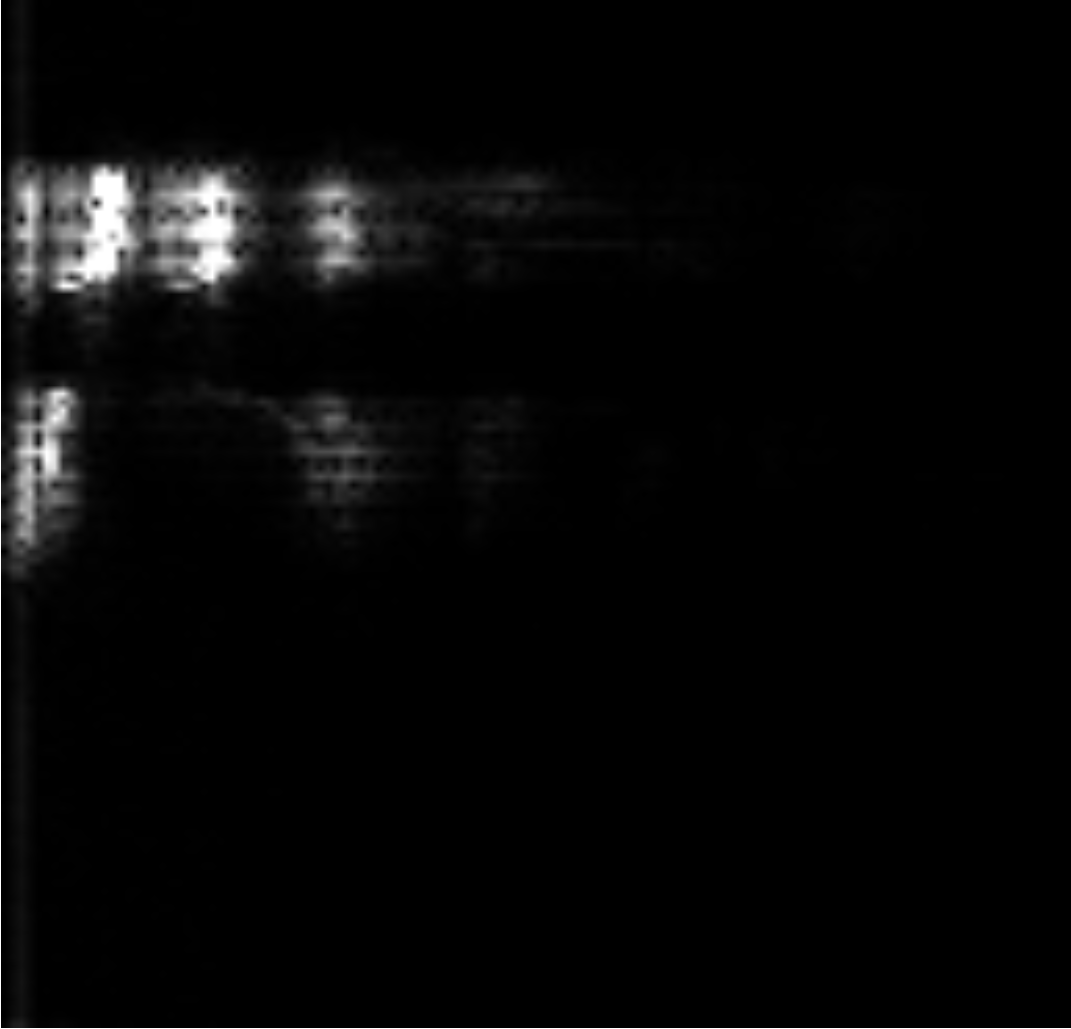
\includegraphics[width=0.7\linewidth]{Rapport2}
	\caption{Spectrogram of one of our sample during the training (image of the Tensorflow website).}
\end{figure}

\hspace*{0.6cm}
In the figure 2.1, time is increasing from top to bottom and frequencies from left to right. We can also different part of the sound that are probably specific part of it (like a syllable in our case of word).\\
\hspace*{0.6cm}
When our image is processed we can then fed it into a  multi-layer convolutional neural network, with a fully-connected layer followed by a softmax at the end.\\
\\
\hspace*{0.6cm}
Now we have a neural network ready to label our words in Pyroomacoustics. It took between 16h-20h to train it and we're going to look at his accuracy later on in this report.


\section{The GoogleSpeechCommand Dataset: Basic informations}
\hspace*{0.6cm}
Created by the tensorflow and AIY teams, the speech command dataset is used to add training and inference in tensorflow. The dataset contains 65,000 one-second long sound of 30 short words, spoke by "thousands of different people". This dataset is not fixed and will continue to increase with the contribution of users. It is designed to help an user to create is own basic voice recognition interface, with common words like 'yes', 'no', directions, etc...\\
\begin{figure}
	\centering
	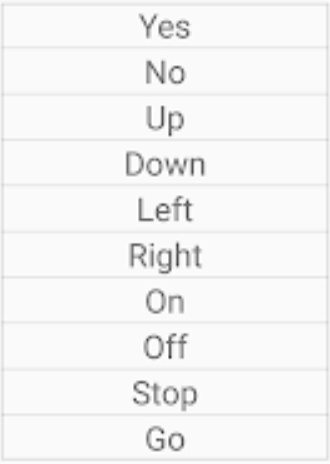
\includegraphics[width=0.5\linewidth]{rapport3}
	\caption{The different words our system is able to recognize}
\end{figure}

\section{Some Signal Processing concepts}
\hspace*{0.6cm}
In this section we're going to talk about one of the most important concept of signal processing we used during this project: the Signal to Noise Ratio (SNR) and everything that comes from it. Even though this concept is quite simple and well known, we will talk about it cause we used it nearly everywhere as you'll see later when we will talk about the implementation (Chapter 4).\\
\hspace*{0.6cm}
First of all, for a single sensor, considering the signal y(t) = s(t) + n(t), with s(t) being the sound of interest and n(t) being the noise, the Signal to Noise Ratio is defined as the sound power over the noise power.
\[SNR\textsubscript{sensor} = \dfrac{E[|s(t)^2|]}{E[|n(t)^2|]} = \dfrac{\sigma\textsubscript{s}^2}{\sigma\textsubscript{n}^2}  \] 
with $\sigma\textsubscript{s}^2$ being the power of the sound of interest and $\sigma\textsubscript{n}^2$ being the power of the noise.\\
Then if we know consider an array of M sensors and define that the signal received at the sensor m is y\textsubscript{m}(t) = s\textsubscript{m}(t) + n\textsubscript{m}(t). We define the signal for the all array Z(t) such that:
\[Z(t) = \sum_{m=0}^{M-1}{w\textsubscript{m}* y\textsubscript{m}(t-\Delta\textsubscript{m})} = Z\textsubscript{s}(t) + Z\textsubscript{n}(t) \]
with w\textsubscript{m} being the weight corresponding to the signal y\textsubscript{m} and $\Delta$\textsubscript{m} being a delay that represents the fact that the sound doesn't arrive at the same moment to each sensor.\\
Now we can write that the SNR value of our signal Z(t) is:
\[SNR\textsubscript{array} = \dfrac{E[|Z\textsubscript{s}(t)^2|]}{E[|Z\textsubscript{n}(t)^2|]} = \dfrac{|\sum_{m}w\textsubscript{m}|^2*\sigma\textsubscript{s}^2} {\sum_{m}|w\textsubscript{m}|^2*\sigma\textsubscript{n}^2} \] 
\hspace*{0.6cm}
Finally in this project we don't use the SNR under this form cause it is not really intelligible and easy to use. So we convert it into decibels (dB) such that we know have:
\[ SNR\textsubscript{dB} = 10\log\textsubscript{10}{\dfrac{\sigma\textsubscript{s}^2}{\sigma\textsubscript{n}^2}} \]

\section{The algorithms}
\hspace*{0.6cm}
In this section we are going to talk about the different algorithm we used in this project.
\subsection{Single Noise Channel Removal}
\hspace*{0.6cm}
The Single Noise Channel Removal is used to suppress the noise. We consider a noisy 
\subsection{Beamforming: Rake Delay and Sum Weights}
\chapter{Implementation}
\section{The GoogleSpeechCommand Dataset}
\section{How to label a file?}
\section{How to synthesize noisy signals}
\section{The algorithms}
\chapter{Results}
\section{Analyse improvement of Single Noise Channel Removal}
\section{Analyse improvement of Beamforming}
\chapter{Conclusion}
\section{Where are we now?}
\section{What's next?}
\chapter{Bibliography}
1) arXiv:1710.04196v1 [cs.SD],
	Robin Scheibler, Eric Bezzam,
		Ivan Dokmanic, \textit{"Pyroomacoustics: a python package for audio room simulation and array processing algorithms"},
	Ecole Polytechnique F�d�rale de Lausanne (EPFL),
		University of Illinois Urbana-Champaign, USA,
	11 Oct 2017
\\
\\
2) Tensorflow,
	\textit{Simple Audio Recognition},
	13 January 2018,
	\url{https://www.tensorflow.org/versions/master/tutorials/audio_recognition}
\\
\\
3) Pete Warden, Software Engineer, Google Brain Team, 
   Google AI Blog,
   \textit{Launching the Speech Command Dataset}
   24 August 2017
   \url{https://ai.googleblog.com/2017/08/launching-speech-commands-dataset.html}
\\
\\
4) J�rgen Grythe, 
	\textit{Array gain and reduction of self-noise}, 
	Norsonic AS, Oslo, Norway,
	2016

\end{document}